\documentclass[preprint,review,12pt]{elsarticle}

\usepackage{amssymb,amsmath}
\usepackage{graphicx}
\usepackage{booktabs}
\usepackage{array}
\usepackage[hyphens]{url}
\usepackage{tikz}
\usepackage{lineno}
\usepackage[colorlinks=true,allcolors=blue]{hyperref}
\usetikzlibrary{arrows.meta,positioning}
\setlength{\emergencystretch}{3em}
\sloppy

\journal{Computer Methods and Programs in Biomedicine}

\begin{document}

\begin{frontmatter}

\title{Reconstructable, privacy-preserving provenance for FHIR-to-large language model clinical transactions: a protocol demonstration}

\author[addr]{Satya Venkata Ranga Janaki Sriram Mentey\corref{cor1}}
\ead{srirammentey@ieee.org}
\cortext[cor1]{Corresponding author. ORCID: 0009-0007-2681-006X.}
\affiliation[addr]{organization={Independent researcher},
  city={Austin},
  state={TX},
  country={USA}}

\begin{abstract}
\noindent\textbf{Background and Objectives:}
Clinical artificial intelligence (AI) systems that consume electronic health
record data and emit reviewer-facing summaries rarely preserve the inputs,
transformations, model configuration, evidence, safeguards, and human
disposition needed to reconstruct a transaction. Storing raw clinical payloads
or hidden model reasoning in an immutable log to fill that gap is unsafe. This
study asks whether one Fast Healthcare Interoperability Resources (FHIR) to
large language model (LLM) transaction can be reconstructed and
integrity-checked without either.

\noindent\textbf{Methods:}
Curie Audit Plane separates protected clinical content from an append-only
audit chain of typed events with content digests. A completed transaction root
is placed in a one-leaf Merkle envelope and signed with Ed25519. Model output is
constrained to structured rationale with evidence references, uncertainty,
assumptions, and missing data; hidden chain-of-thought fields are rejected. A
versioned harness reloads persisted records, runs a separate verifier module,
applies 19 labeled mutations, ablates provenance classes, probes role-based
access, and measures capture overhead against an identical unrecorded clinical
workflow.

\noindent\textbf{Results:}
On synthetic FHIR Release~4 fixtures, reload-and-verify audit reconstruction
completeness was 20 of 20 required fields. All 19 mutations produced a
non-verified outcome (18 tampered, one incomplete), and 11 of 11 access probes
matched their expected outcome. Complete capture added 103\% mean latency
(16.1 versus 8.6\,ms; 95\% interval 79--128\%) and a 3.5-fold logical storage
multiplier (7.2-fold allocated on disk).

\noindent\textbf{Conclusions:}
A data/proof split makes a bounded FHIR-to-LLM handoff reconstructable without
placing raw protected health information or hidden reasoning in an immutable
store. The contribution integrates known integrity and interoperability
primitives into application software; overhead is substantial at
single-transaction scale, and clinical or population-scale evaluation remains
future work.
\end{abstract}

\begin{keyword}
Fast Healthcare Interoperability Resources \sep
Provenance \sep
Audit trail \sep
Large language models \sep
Data integrity \sep
Biomedical informatics
\end{keyword}

\end{frontmatter}

\linenumbers

\section{Introduction}
\label{sec:intro}

Large language models are being attached to electronic health record
workflows for summarization and review support. Healthcare organizations still
need a narrower answer: given one completed transaction, can an investigator
reconstruct what the model was shown, how it was configured, which evidence
and safeguards were applied, and what a human reviewer decided, without
placing raw protected health information or hidden reasoning into an immutable
store?

This paper treats that question as application-software design for
biomedical informatics, not as generic logging and not as a clinical efficacy
trial. The prototype is deliberately narrow: one synthetic FHIR Release~4
encounter, one structured clinical-summary task, and a human
ACCEPT/MODIFY/REJECT disposition. It is a protocol and software demonstration
on synthetic fixtures, not a population study or a claim of readiness for
regulatory use.

The research questions, fixed before measurement, are: (i)~reconstructability
of required provenance fields; (ii)~detection of mutation, omission,
reordering, broken references, and invalid proofs; (iii)~latency and storage
overhead of complete capture versus an identical unrecorded clinical workflow;
(iv)~console exposure of evidence, uncertainty, guardrail results, and
disposition, demonstrated with a scripted proxy (\texttt{SCRIPTED\_PROXY})
rather than a blinded reviewer study; and (v)~replay fidelity for a
deterministic stub versus a hosted nondeterministic model.

The contribution is an integration: a data/proof split, typed events,
structured rationale without hidden chain-of-thought, FHIR
\texttt{Provenance}/\texttt{AuditEvent} projections, and reload-and-verify
scoring against construct-dependent analytical baselines, released as
reproducible open-source software. Hash chaining, Merkle trees, and Ed25519
are used as known primitives, not as new cryptographic
results~\cite{haber1991timestamp,merkle1988signature,rfc8032}.

\subsection{Related work}
\label{sec:related}

Healthcare audit and provenance already have native interoperability
surfaces. FHIR \texttt{Provenance} and \texttt{AuditEvent} record agents,
entities, and access events, and W3C PROV-DM supplies a generic provenance
data model~\cite{hl7provenance,hl7auditevent,provdm}. IHE Audit Trail and Node
Authentication addresses node-level audit trails and secure communication in
clinical networks~\cite{ihe-atna}. FHIR implementation surveys and the FHIR
security framework document how these resources are used in
practice~\cite{ayaz2021fhir,hl7security}. These artifacts are necessary
interoperability projections, but they are not, by themselves, an internal
event chain that can reconstruct a FHIR-to-LLM handoff: input manifests,
transformations, prompt and model identity, retrieved evidence digests,
guardrail outcomes, and human disposition.

Tamper-evident logging has a long cryptographic literature. Haber and
Stornetta time-stamped documents with hash-linked records; Merkle trees supply
inclusion proofs; Schneier and Kelsey and Crosby and Wallach developed
hash-chained and efficient tamper-evident logs; and Certificate Transparency
uses Merkle trees for publicly auditable
logs~\cite{haber1991timestamp,merkle1988signature,schneier1998logs,crosby2009tamper,rfc6962}.
This prototype composes those primitives in a local append-only store. It is
not a distributed ledger and is not evaluated against blockchain-in-healthcare
architectures~\cite{agbo2019blockchain}.

Clinical LLM evaluation has focused mainly on accuracy, fairness, and the
limits of electronic-health-record foundation
models~\cite{wornow2023shaky,bedi2025testing}. Adapted models can outperform
experts on clinical text summarization, and LLMs encode substantial clinical
knowledge, but those results do not address transaction
auditability~\cite{vanveen2024adapted,singhal2023medpalm}. A systematic review
of 519 health-care LLM studies found that almost all used accuracy as the
primary dimension and that deployment considerations were rarely
measured~\cite{bedi2025testing}. Clinical AI governance work, including model
cards, model-facts labels, and good machine learning practice, describes
intended use and performance~\cite{mitchell2019modelcards,sendak2020modelfacts,fda2021gmlp};
it does not record the inputs, evidence, guardrails, and human disposition of
one completed transaction.

\section{Methods}
\label{sec:method}

\subsection{System boundary}
\label{sec:boundary}

Curie Audit Plane observes a synthetic FHIR-to-LLM workflow
(Fig.~\ref{fig:boundary}). Protected payloads (assembled context, model
request and response, reviewer-modified text, and free-form comments) are
stored in an authorized content store. The immutable audit store holds
metadata, opaque references, schemas, and digests. Reviewer comments on the
chain are limited to a controlled category; detailed text is protected.
Provider exception text is neither stored nor fingerprinted. Patient and
resource identifiers in immutable metadata are opaque tokens; a protected
identity map is required for authorized reconstruction.

\begin{figure}[t]
\centering
\resizebox{0.85\textwidth}{!}{%
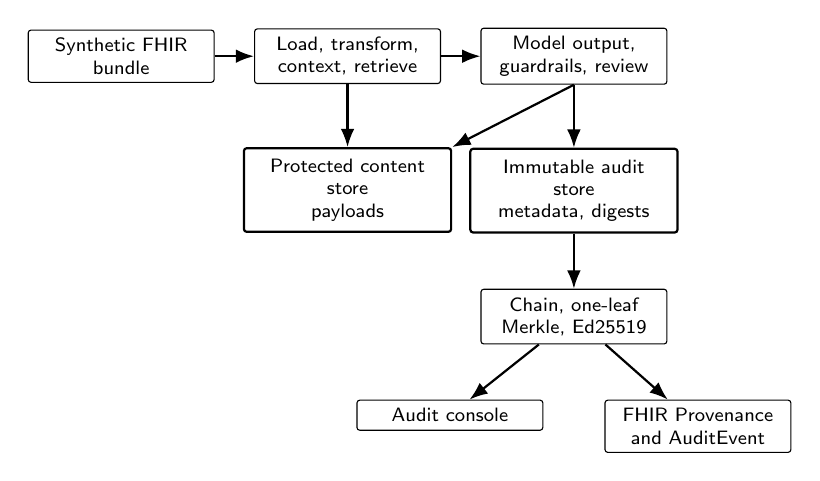
\begin{tikzpicture}[
  font=\scriptsize\sffamily,
  box/.style={draw, rounded corners=1pt, align=center, inner sep=3pt, text width=2.15cm},
  store/.style={draw, thick, rounded corners=1pt, align=center, inner sep=4pt, text width=2.35cm},
  arr/.style={-{Latex}, thick}
]
\node[box] (fhir) {Synthetic FHIR\\bundle};
\node[box, right=5mm of fhir] (stages) {Load, transform,\\context, retrieve};
\node[box, right=5mm of stages] (llm) {Model output,\\guardrails, review};
\draw[arr] (fhir) -- (stages);
\draw[arr] (stages) -- (llm);
\node[store, below=8mm of stages] (prot) {Protected content\\store\\payloads};
\node[store, below=8mm of llm] (audit) {Immutable audit\\store\\metadata, digests};
\draw[arr] (stages.south) -- (prot.north);
\draw[arr] (llm.south) -- (prot.north east);
\draw[arr] (llm.south) -- (audit.north);
\node[box, below=7mm of audit] (proof) {Chain, one-leaf\\Merkle, Ed25519};
\draw[arr] (audit) -- (proof);
\node[box, below left=7mm and -8mm of proof] (ui) {Audit console};
\node[box, below right=7mm and -8mm of proof] (fhirp) {FHIR Provenance\\and AuditEvent};
\draw[arr] (proof) -- (ui);
\draw[arr] (proof) -- (fhirp);
\end{tikzpicture}}
\caption{System boundary. Protected clinical payloads stay outside the
immutable audit store. The measured path signs one completed transaction root
per Merkle envelope.}
\label{fig:boundary}
\end{figure}

\subsection{Event model and integrity}
\label{sec:events}

A successful transaction emits typed events from input manifestation through
human action and an integrity-proof commitment. Events are canonically hashed
and chained. The completed transaction root is represented as a one-leaf
Merkle envelope and signed with Ed25519; the measured pipeline does not
aggregate multiple transaction roots into one batch. Verification reports
\texttt{VERIFIED}, \texttt{INCOMPLETE}, \texttt{TAMPERED}, or \texttt{FAILED}.
The verifier is a separate module in the same repository, run after persisted
SQLite and protected-content records are reloaded; it is not an external
third-party audit. Access and export events are written to a separate
hash-chained access-audit stream, so reading a sealed transaction does not
alter its clinical proof. FHIR Release~4 \texttt{Provenance} and
\texttt{AuditEvent} resources are documented projections of the internal
model, not a validated Implementation Guide profile.

\subsection{Structured output and guardrails}
\label{sec:guardrails}

Model output must validate as structured rationale. Guardrails record schema
validity, evidence-reference coverage, uncertainty presence, a synthetic
identifier scan, and policy action. Blocking results require an explicit
override policy before ACCEPT. Hidden chain-of-thought fields are rejected at
the schema boundary.

\subsection{Software implementation}
\label{sec:software}

The system is implemented in Python with a FastAPI service, SQLite audit and
protected-content stores, and a React audit console that presents an event
timeline, formatted and raw JSON, verification scope, and an artifact-count
flow view. API endpoints are role-gated (reviewer, investigator, admin) with
locally generated bearer tokens. The reproducible entry point is
\texttt{curie-audit-plane evaluate}.

\subsection{Evaluation protocol}
\label{sec:eval}

Reports use schema \texttt{curie-evaluation.v1.1} and record experiment
metadata (git commit, dirty-tree flag, fixture alias and digest, provider,
model, prompt version, decoding parameters, endpoint class, seed, and command
template) without absolute local paths.

The headline metric, audit reconstruction completeness (ARC), is the fraction
of 20 required provenance fields present after reloading persisted records,
counted only when the verifier succeeds (report field
\texttt{independently\_verified\_arc}). Field-presence completeness on the
in-memory object is reported separately. Mutation detection uses 19 labeled
cases; a case is detected when the verifier returns any
non-\texttt{VERIFIED} status, and the specific status is reported. Replay is
classified as \texttt{EXACT\_MATCH}, \texttt{EQUIVALENT}, or
\texttt{DIVERGENT}.

Overhead compares the complete plane with an identical unrecorded clinical
workflow (load, transform, context, retrieve, complete, guardrails, and an
in-memory ACCEPT disposition written only to JSONL) on isolated stores, with
one warmup and 30 timed repeats. The unrecorded path emits no audit events,
Merkle proofs, or signatures.
\begin{align}
\mathrm{overhead}_{\mathrm{latency}} &= (T_{\mathrm{plane}}-T_{\mathrm{no\_audit}})/T_{\mathrm{no\_audit}}, \\
\mathrm{storage\ multiplier} &= B_{\mathrm{plane}}/B_{\mathrm{no\_audit}}.
\end{align}
Allocated bytes are on-disk file sizes, including SQLite page allocation.
Logical bytes are UTF-8 octet lengths of serialized event JSON,
transaction-row payloads, and protected-content files, excluding page
padding. Rate metrics use Wilson intervals.

Ablations omit input manifests, transformations, model and prompt metadata,
evidence references, cryptographic proofs, or human provenance.
Access-control probes record allowed and denied HTTP outcomes for reviewer,
investigator, admin, output, content, export, missing transaction, and global
list scope. The comparison recorders (application JSONL, hash-only JSONL, and
a FHIR R4 projection) are analytical emulations built for this study and
scored against the same required-field inventory; they are not independently
shipped products.

The default 50-encounter cohort rewrites one synthetic fixture; it tests
repeatability of a single workflow, not a population. Optional Synthea
slices~\cite{walonoski2018synthea} are excluded from measured evidence because
generator version, seed, module set, and command line are not pinned.

\subsection{Threat model}
\label{sec:threat}

Adversaries may mutate, delete, or reorder events; substitute proofs or keys;
present unsupported findings; or attempt to place protected health
information in reviewer comments, provider errors, research exports, or
endpoint configuration. The prototype assumes synthetic data, local keys, and
an approved loopback model endpoint. It does not protect against compromised
signing keys or a malicious protected-content store operator.

\section{Results}
\label{sec:results}

All numbers are from the deterministic-stub evaluation report in
\texttt{evaluation-results/} (schema \texttt{curie-evaluation.v1.1}, git commit
\texttt{0dcf801}, clean working tree), archived under tag
\texttt{jbhi-eval-20260828}. At that commit the repository had 146 Python
tests, 94.59\% statement coverage, and a clean linter pass; these are software
quality indicators, not clinical performance.

\subsection{Reconstructability and tamper detection}

ARC was 20/20 required fields on the clean fixture transaction after the
verifier succeeded; field-presence completeness on the in-memory object was
also 20/20, and required-event completeness was 11/11. All 19 labeled
mutations produced a non-\texttt{VERIFIED} result: 18 were classified
\texttt{TAMPERED}, and one substituted content reference was classified
\texttt{INCOMPLETE} because the referenced protected content was absent. The
false-tamper rate over three clean runs was 0. Verification of the clean
transaction took 1.55\,ms. Across the 50-encounter cohort, ARC,
required-event completeness, and human-action capture were each 50/50 (Wilson
95\% interval 0.93--1.00), with mean verification latency 1.21\,ms.

\begin{table}[t]
\centering
\caption{Comparison recorders on the synthetic fixture. Scores use this
paper's required-field inventory and are construct-dependent.}
\label{tab:baselines}
\begin{tabular}{lccc}
\toprule
Recorder & ARC & Tamper detection & Queryability \\
\midrule
Application JSONL & 0.10 & 0.00 & 0.00 \\
Hash-only JSONL & 0.15 & 1.00 & 0.00 \\
FHIR R4 projection & 0.20 & 0.00 & 0.25 \\
Complete plane & 1.00 & 1.00 & 1.00 \\
\bottomrule
\end{tabular}
\end{table}

The complete plane reconstructs more required fields and detects the standard
model-event mutation that application logs and FHIR projections do not
(Table~\ref{tab:baselines}). Hash-only logging detects digest mismatch without
chain or signature guarantees. These gaps are expected by construction: the
comparison recorders were not designed to capture the same field set.

\subsection{Ablations}

Table~\ref{tab:ablation} reports ARC after omitting one provenance class.
Omitting cryptographic proofs has the largest effect (0.75), followed by
human provenance (0.85) and model and prompt metadata (0.90). These are
field-presence ablations, not clinical-efficacy ablations.

\begin{table}[t]
\centering
\caption{Audit reconstruction completeness after omitting a provenance class.}
\label{tab:ablation}
\begin{tabular}{lcc}
\toprule
Condition & ARC & $\Delta$ from full \\
\midrule
Full recorded provenance & 1.00 & 0.00 \\
Omit input manifests & 0.95 & 0.05 \\
Omit transformations & 0.95 & 0.05 \\
Omit model and prompt metadata & 0.90 & 0.10 \\
Omit evidence references & 0.95 & 0.05 \\
Omit cryptographic proofs & 0.75 & 0.25 \\
Omit human provenance & 0.85 & 0.15 \\
\bottomrule
\end{tabular}
\end{table}

\subsection{Access control}

Eleven role probes returned the predeclared HTTP status (11/11; Wilson 95\%
interval 0.74--1.00): reviewer read and output allowed; reviewer export and
investigator output or content denied; investigator verify and export
allowed; admin content allowed; unauthenticated list denied (401); missing
transaction reported as missing (404); and global list allowed.

\subsection{Overhead and replay}

\begin{table}[t]
\centering
\caption{Capture overhead versus an identical unrecorded workflow ($n=30$
paired runs for latency).}
\label{tab:overhead}
\begin{tabular}{lrrr}
\toprule
Measure & Plane & Unrecorded & Ratio \\
\midrule
Mean latency (ms) & 16.13 & 8.59 & +103.3\% \\
Allocated storage (bytes) & 81\,885 & 11\,373 & $7.20\times$ \\
Logical storage (bytes) & 39\,454 & 11\,373 & $3.47\times$ \\
\bottomrule
\end{tabular}
\end{table}

Complete capture roughly doubled latency (Table~\ref{tab:overhead}; mean
paired relative overhead +103.3\%, 95\% interval +78.8\% to +127.8\%). The
allocated audit file was a single 65\,536-byte SQLite page holding 23\,105
logical bytes of events and transaction rows, so page allocation inflates the
on-disk multiplier; the logical multiplier (3.47) is the less confounded
figure. These results do not support a claim of low overhead at
single-transaction scale. Deterministic-stub same-prompt replay was exact, and
prompt-substitution replay was \texttt{DIVERGENT} by construction. The one
hosted same-prompt replay observation was \texttt{DIVERGENT} ($n=1$); no
hosted replay rate is estimated.

A 16-arm scenario matrix exercised ACCEPT/MODIFY/REJECT, forced and natural
WARN/BLOCK guardrail outcomes, provider failure, a sparse encounter, MODIFY
evidence, prompt-substitution replay, and access audit. It demonstrates
workflow coverage rather than sampling a population; the two unpinned Synthea
arms are excluded from the measured tables. Fig.~\ref{fig:console} shows the
console surfaces used in the scripted reconstruction demonstration.

\begin{figure}[t]
\centering
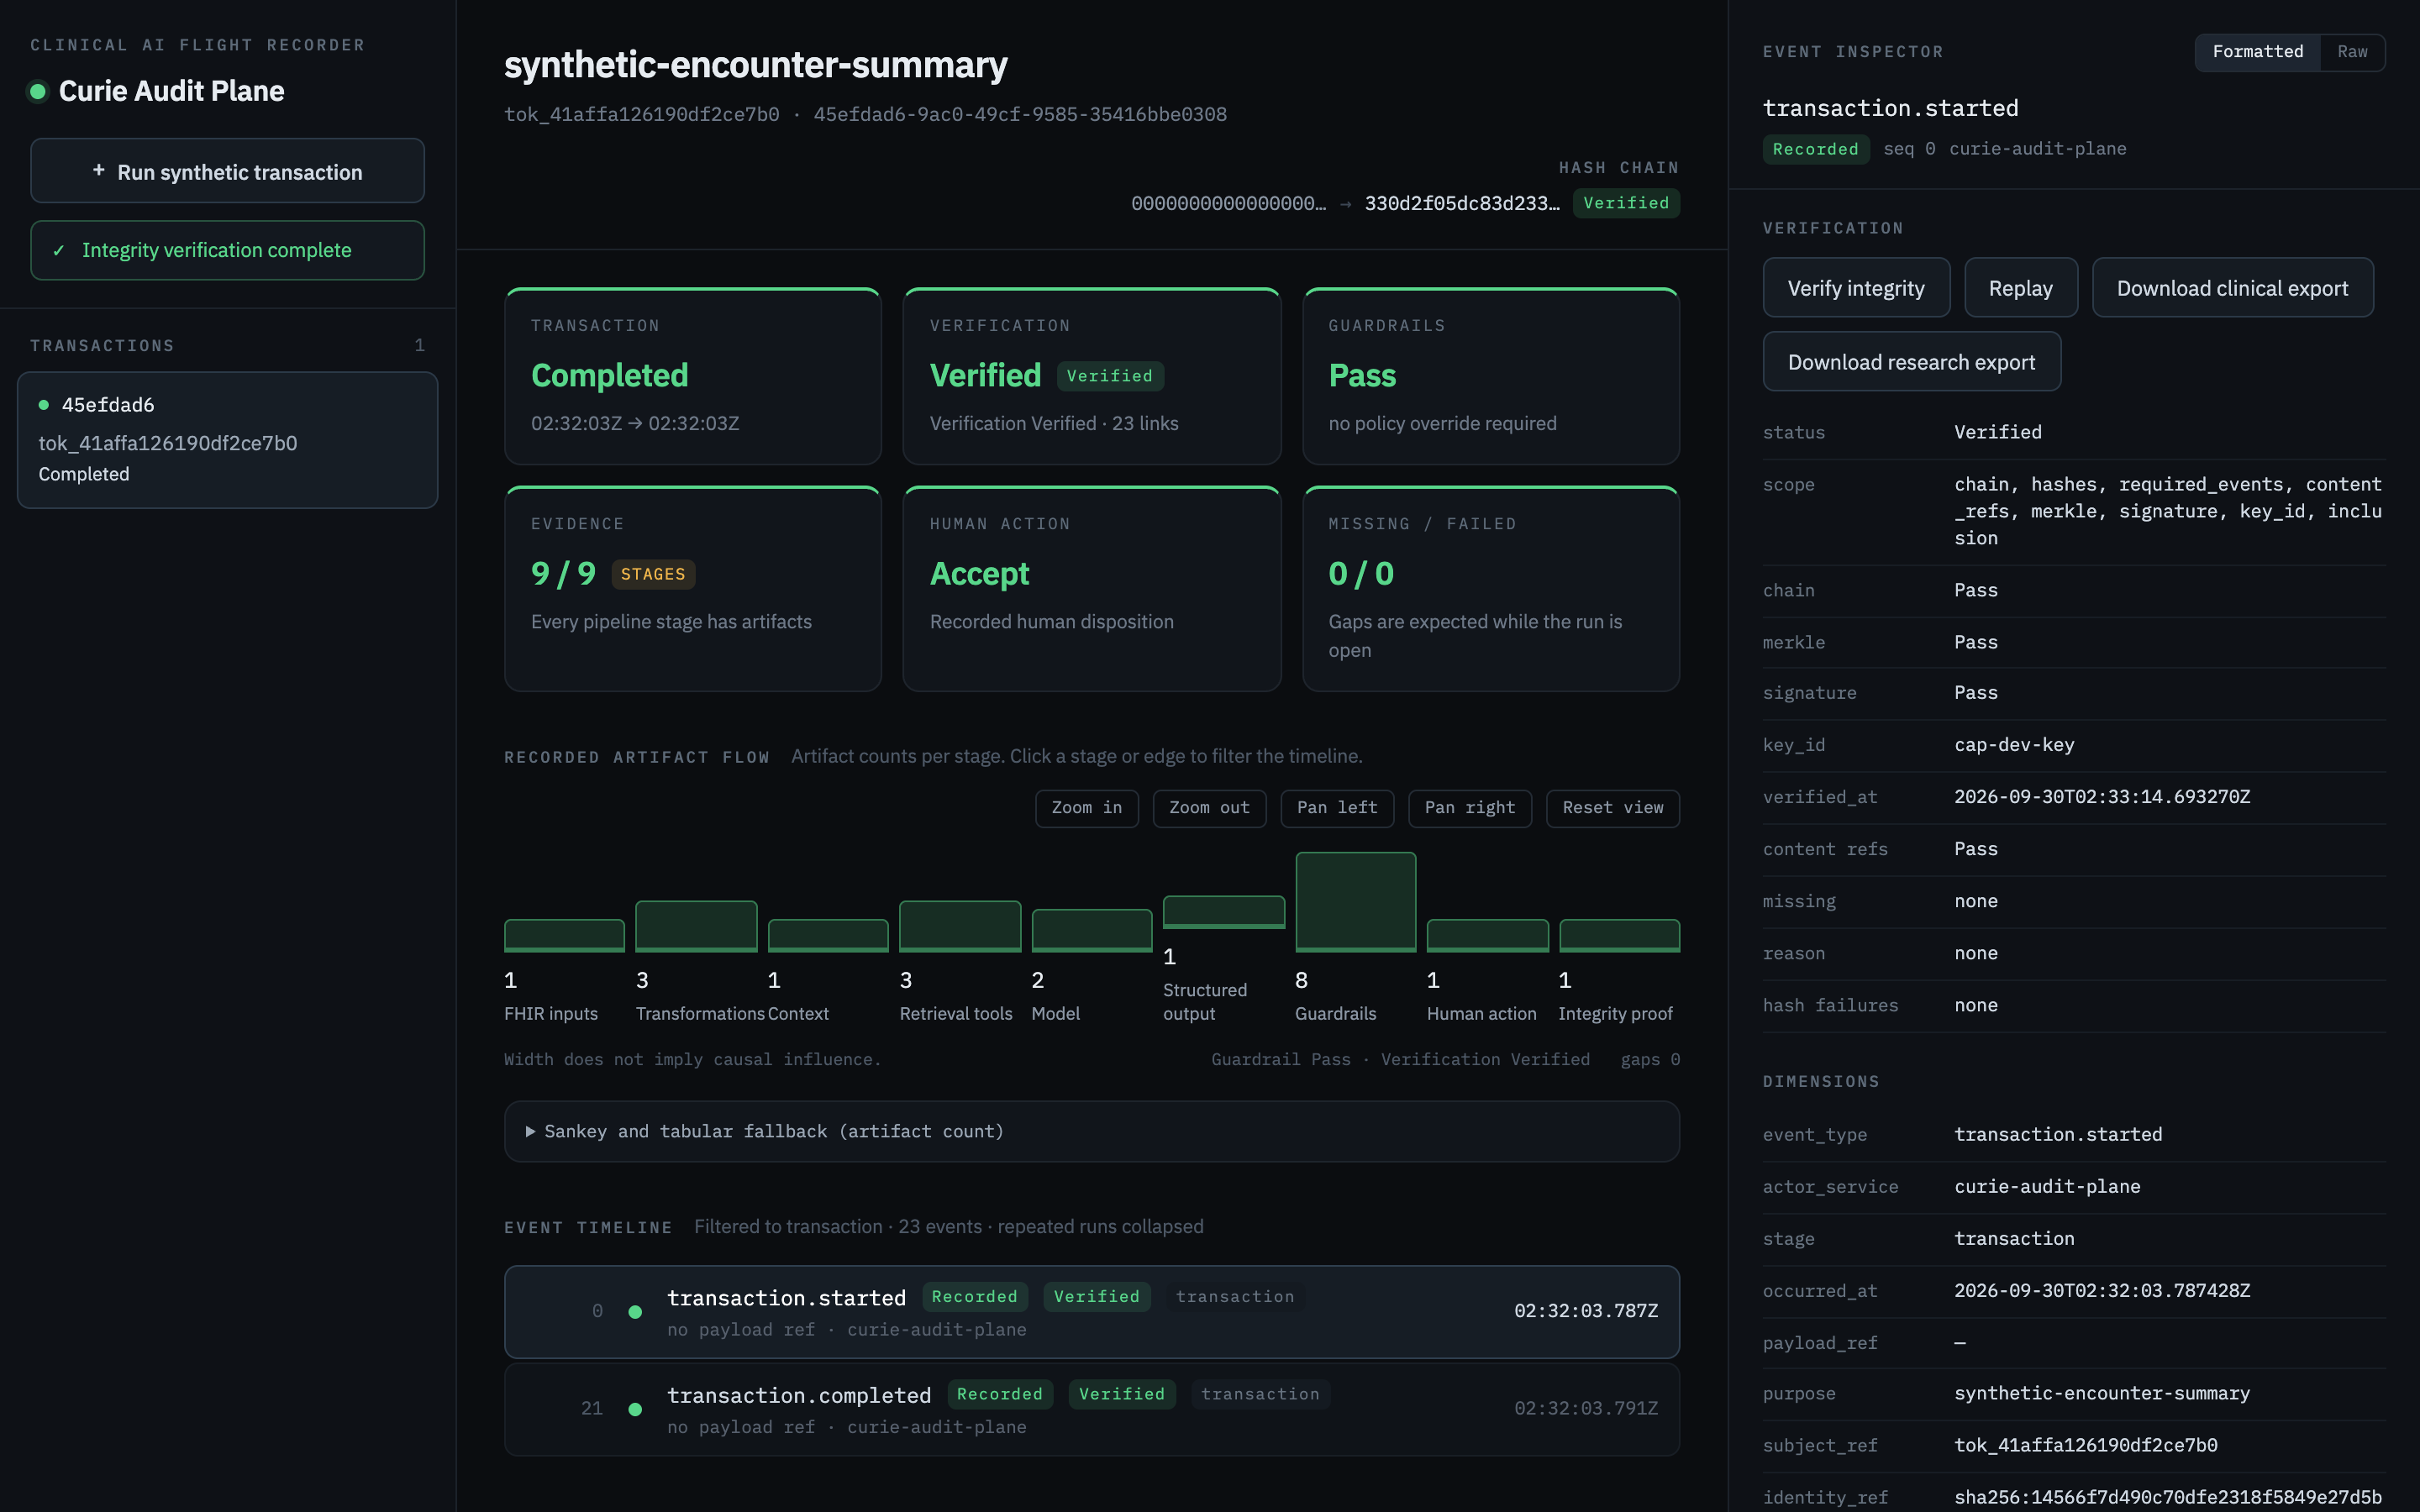
\includegraphics[width=\textwidth]{figures/console-overview.png}
\caption{Audit console on a synthetic transaction after integrity
verification: overview tiles, recorded artifact-count flow (width does not
imply causal influence), event timeline, and verification scope with chain,
Merkle, signature, and content-reference checks. The subject is shown only as
an opaque token.}
\label{fig:console}
\end{figure}

\section{Discussion}
\label{sec:discussion}

In an electronic health record setting the plane would sit beside an existing
FHIR access path rather than replace it. A hospital integration would continue
to enforce resource authorization in the clinical system, store protected
payloads under that authority, and emit the typed audit events described
here, with FHIR \texttt{Provenance} and \texttt{AuditEvent} as the
interoperability projection for downstream governance tools. The design keeps
the LLM off any deterministic alert-firing path, and reconstructability does
not imply clinical correctness.

The ablations indicate where the reconstruction value lies: cryptographic
proofs and human provenance account for the largest share of required fields,
which is the information ordinary application logs and FHIR projections most
often lack. The overhead results are the main practical cost. At one
transaction per Merkle envelope, fixed per-transaction work (signing,
chaining, page allocation) dominates; batching multiple roots per envelope is
the obvious amortization path but was not evaluated.

\subsection{Limitations}
\label{sec:limitations}

This is a single-workflow protocol demonstration on synthetic FHIR fixtures.
The cohort rewrites one fixture and is not 50 independent patients. Baseline
scores are construct-dependent, measured against analytical emulations rather
than shipped logging products. The verifier is in the same repository, not an
external audit. Each Merkle envelope holds one transaction, so batching and
multi-transaction storage amortization are unreported. Latency with $n=30$ is
an overhead estimate, not a capacity or tail-latency study. FHIR projections
are mapping rules without Implementation Guide validation. Console
reconstruction was demonstrated with a scripted proxy, not with clinicians or
auditors.

\subsection{Conclusions}
\label{sec:conclusion}

A privacy-preserving provenance plane can reconstruct a bounded synthetic
FHIR-to-LLM transaction from persisted records, detect a defined mutation
suite, and keep hidden reasoning and free-form reviewer text out of the
immutable chain, at the cost of roughly doubled latency and a 3.5-fold logical
storage multiplier at single-transaction scale. The result integrates known
primitives under a clinical data/proof split; it is not a new integrity
scheme or a population evaluation. Next steps are independent synthetic
patients at scale, batched envelopes, hosted-model replay characterization,
and a reconstruction study with clinical auditors.

\section{Acknowledgements}
\label{sec:ack}

The author received no external funding and no assistance from a
professional editor. Use of AI tools is disclosed below.

\section*{Ethics}
No human subjects or identifiable clinical records were used. The evaluation
uses synthetic FHIR templates; therefore no institutional review board
approval was required.

\section*{Funding}
This research did not receive any specific grant from funding agencies in the
public, commercial, or not-for-profit sectors.

\section*{Declaration of competing interest}
The author declares no known competing financial interests or personal
relationships that could have appeared to influence the work reported in this
paper.

\section*{Data and code availability}
Source code, synthetic fixtures, and versioned evaluation artifacts are
openly available at \url{https://github.com/sreeram843/curie-audit-plane}
under tag \texttt{jbhi-eval-20260828}. No patient data were used.

\section*{CRediT authorship contribution statement}
\textbf{Satya Venkata Ranga Janaki Sriram Mentey:} Conceptualization,
Methodology, Software, Validation, Formal analysis, Investigation, Data
curation, Writing -- original draft, Writing -- review \& editing,
Visualization.

\section*{Declaration of generative AI and AI-assisted technologies in the writing process}
During the preparation of this work the author used AI coding agents to draft
portions of the software and documentation and to assist with manuscript
editing. All evaluation metrics were produced by the versioned Python harness.
After using these tools, the author reviewed and edited the content as needed
and takes full responsibility for the content of the publication.

\bibliographystyle{elsarticle-num}
\bibliography{references}

\end{document}
